\documentclass[12pt,a4paper,oneside,article]{memoir}

\usepackage{polyglossia}
\setdefaultlanguage{english}
\usepackage{fontspec}

\defaultfontfeatures{Ligatures=TeX}
\newfontfeature{Microtype}{protrusion=default;expansion=default}
\usepackage[final]{microtype}
\setmainfont{Linux Libertine O}
\setsansfont{Linux Biolinum O}
\setmonofont{DejaVu Sans Mono}

\usepackage{subfiles}
\usepackage{tabularx}
\usepackage{tabu}
\usepackage{booktabs}
\usepackage{multirow}
\usepackage{float}
\usepackage{amsmath,amsfonts,amssymb}
\usepackage{mathtools}
\usepackage[shortlabels]{enumitem}

\usepackage{tikz}
\usepackage{graphicx}
\usepackage{hyperref}
\hypersetup{hidelinks}
\usepackage{xcolor, colortbl, array}

\usepackage{listings}
\usepackage{color}
\lstset{
  language=Python,
  frame=tb,
  breaklines=true,
  breakatwhitespace=true,
  keepspaces=true,
  columns=fullflexible,
  showspaces=false,
  showstringspaces=false,
  showtabs=false,
  basicstyle=\ttfamily\footnotesize
}

\usepackage[autostyle,strict,autopunct]{csquotes}
\usepackage[style=ieee,backend=biber]{biblatex}
\bibliography{bibliography}

\usepackage{chngcntr}
\counterwithin{table}{section}
\numberwithin{equation}{chapter}
\counterwithin{figure}{section}
\setenumerate[0]{label= (\alph*)}
\AtBeginDocument{\counterwithin{lstlisting}{section}}
\counterwithout{section}{chapter}

\chapterstyle{hangnum}
\pagestyle{ruled}

\title{MOCCA: MOCCA Operational Controller for Coffee Availability}
\author{Eivind D. Halderaker, Sondre Å. Nilsen}
\date{Spring 2019}
\begin{document}

\begin{titlepage}

\newcommand{\HRule}{\rule{\linewidth}{0.5mm}} % Defines a new command for the 
%horizontal lines, change thickness here

\center % Center everything on the page
 
%-------------------------------------------------------------------------------
%---------
%	HEADING SECTIONS
%-------------------------------------------------------------------------------
%---------

\textsc{\LARGE University of Bergen \\ Department of informatics}\\[1.5cm] % 
%Name of your university/college

%-------------------------------------------------------------------------------
%---------
%	TITLE SECTION
%-------------------------------------------------------------------------------
%---------

\HRule \\[0.5cm]
\begin{Huge}
	\bfseries{MOCCA: MOCCA Operational Controller for Coffee 
Availability}\\[0.7cm] % Title of your document
\end{Huge}
\HRule \\[0.5cm]

%-------------------------------------------------------------------------------
%---------
%	AUTHOR SECTION
%-------------------------------------------------------------------------------
%---------

\large \emph{Author:} Eivind D. Halderaker, Sondre Å. Nilsen\\
\large \emph{Supervisor:} Lars Albin Severinson\\[2cm]

%-------------------------------------------------------------------------------
%---------
%   LOGO SECTION
% 	This will require the graphicx package
%	Change the line to comment if you only want the UiB Logo
%	Logo for other faculties here: 
% http://kapd.h.uib.no/profilmanual/99LastNed/99a_lastned.html
%-------------------------------------------------------------------------------
%---------

\centerline{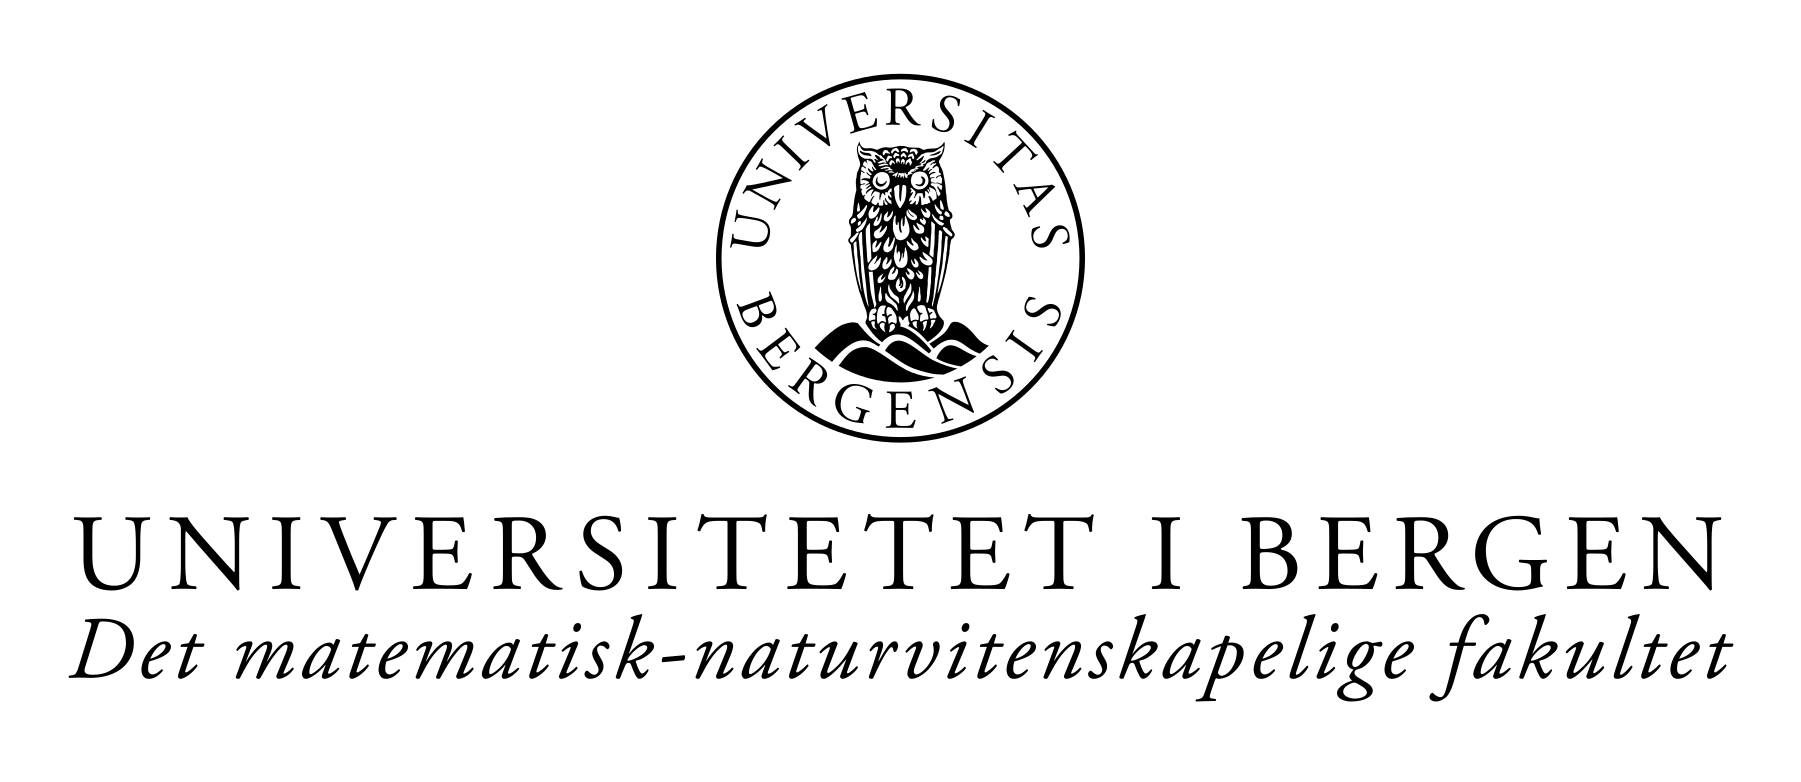
\includegraphics[scale=1.9]{figures/canvasWithFaculty}}
%\centerline{
\includegraphics[scale=0.15]{figures/canvas}}  %change for your 
%faculty

%-------------------------------------------------------------------------------
%---------
%	DATE SECTION
%-------------------------------------------------------------------------------
%---------

{\large Spring 2019}\\[3cm] % Date, change the \today to a set date if 
%you want to be precise

%-------------------------------------------------------------------------------
%---------
%	LOGO SECTION
%-------------------------------------------------------------------------------
%---------

\vfill % Fill the rest of the page with whitespace

\end{titlepage}

\tableofcontents

\begin{abstract}
  As students with access to free coffee in our study hall our biggest problem
  is never knowing whether there will be fresh coffee available from it in times
  of need. \textit{MOCCA} is an attempt to address and fix this problem once and
  for all: a single source of truth about the availability of fresh coffee.
\end{abstract}

\section{Todos}
\begin{itemize}
\item List of acronyms/synonyms/glossary
\item Links/references to technologies/frameworks
\item Sensors requires proper names and so on
\item Give thanks to everyone who has helped
\end{itemize}

\section{Introduction}\label{sec:introduction}
(...) It's an attempt to both write and wire together a solution that combines 
hardware and software to solve a long
standing problem we've had in our study hall. The coffee machine is probably the
most prized and valuable piece of comfort that we have, and is used from eight
in the morning until the last student goes home.

The problem is that you're never sure whether or not there is actually
coffee available, and whenever there is none you waste precious minutes in the
couch waiting for it to finish brewing. There have been many attempts at solving
this problem throughout the years, none of which have survived past the initial
testing phase. This project breaks the chain and have a working product
that can withstand the test of time.

In this report, we describe a system combining different sensors together with 
an Arduino and a Raspberry Pi to monitor a Moccamaster and service 
an API. We call this system \textit{MOCCA}. It's task is to measure both the 
quality and quantity of coffee. 

For quality we use both a temperature sensor 
and power current sensor (?). The temperature is essential to high quality 
coffee, since you do not want it chilled down and definitely not warmed 
up again. Another factor of quality is the age of the brew. The good taste of 
coffee deteriorates as time goes on if it has been held warm for some time. To 
measure the age of a brew we monitor the amount of power the Moccamaster is 
draining. A Moccamaster has essentially three states: turned off, brewing, 
and warming. By saving a time stamp at the start of a new brew, it is trivial 
to calculate age.

Quantity on the other hand is done by image processing. Images are taken of the 
coffee pot and in turn analysed with regards to the amount of dark pixels. 
Taking the background of the pot into account, we produce an rough estimate of 
the amount of coffee. 


\section{System overview}\label{sec:technical-details}

\subsection{DIAGRAM - PLS DO}
\textit{MOCCA} is written in a wide range of languages and technologies, the
back-end is written in Python using the Django framework while the front-end is
written in React, while communication between these two happens across a REST
API.
The most important piece of software and hardware however is the Arduino
that is --- essentially --- our interface, together with the camera on the 
Raspberry Pi, between the real world and our software. It reads the temperature 
of the coffee and how much power the machine is drawing. Without these sensors 
and the camera to interface the Moccamaster the whole system is meaningless. 

Python was chosen for the back-end. It is a programming language with plenty of 
libraries available and is fairly concise. The choice of Django however was a 
bit more contentious, in the very beginning the battle plan was to use Flask 
which would've meant that we'd have to do a lot of the heavy lifting ourselves.
After a fairly quick trial period where we developed a few prototypes the choice
fell on Django, mostly due to the batteries-included approach of it but perhaps
mostly due to Sondre's familiarity with it given he had previous experience with
it.

Thanks to Django we were able to build on top of existing battle-tested
libraries, we used Django REST Framework for the heavy lifting of implementing
the API, we used drf-yasg (Django REST Framework - Yet Another Swagger
Generator) for creating Swagger documentation of the API. For communicating with
our Arduino we used Pyserial and for asynchronously polling it we used Celery.

\subsection{Data collection}\label{sec:data-collection}
\subsubsection{Arduino}\label{sec:arduino}
The code for the Arduino is very simple in all honesty, but it does the job
required. Any code on an Arduino runs in a tight loop that continuously reads
from its sensors and saves the data to a queue. Since we read from the Arduino
every ten seconds, we only want the latest data but we don't want to block
getting the data on the Arduino itself reading its sensors. The way we worked
around this issue was to have the Arduino continuously read to the queue,
discarding the last item in it for every reading, while waiting for us to send a
predetermined message saying that we are ready for data. In our case this
message is simply ``1''.

Once the Arduino receives this it enters a write-mode --- in a sense --- and
fetches the latest reading from the queue, returns it, clears the queue and
exits the current state returning to reading data. The sensors themselves all
came with ready-made libraries that you simply need to download, import them and
then call the documented functions and you are good to go.


\subsection{Raspberry Pi}\label{sec:raspberry-pi}
Raspberry Pi is a small computer with the basics you need: USB, HDMI, WiFi, 
and, most important for us, support for a camera. Though lacking in 
computational power it's size and affordability makes it a perfect data 
cruncher for our case. The Pi can fit in a compact container near the 
Moccamaster. We used Raspberry Pi's very own camera module for ease of use and 
it's included library. The module itself is plug-and-play and has more than high 
enough resolution for our use. We only need a rough estimate of how full the 
coffee pot is and high resolution means more data needed to be processed. Most 
of which is redundant. 
% To be continued...

\section{Software}\label{sec:software}
\subsection{Back-end}\label{sec:back-end}
The back-end is definitely the most complex part of the project, in part because
the real world is messy, but also because you have to orchestra a service that
communicates with the Arduino while also serving an API, which required us to do
the data fetching in the background in a asynchronous task runner.

As mentioned, the real world is messy --- there are a ton of moving parts,
variables and ``states'' it can be in. When reading from the sensors, how do you
know if the current ``state'' of the world is in order? For instance, the coffee
machine can be powered off by two different parts: its own power supply, but
also the power plug itself as it runs on a timer. When getting the power status
from the Arduino, how do you ensure that the machine has been in a consistent
phase and the reading you are getting is not a one-time event? The amount of
possible things you have to account for is near endless, and we have most
definitely not been able to foresee or cover for all of them.

\subsection{Front-end}\label{sec:front-end}
The hardest part of the front-end was definitely the CSS.  Though the least 
complex of the two -ends, it still had its own fair
share of minor issues. We decided early on with using React due to its
popularity for web applications nowadays as a learning experience. React is in
many ways the exact opposite of Django, no batteries included but the ecosystem
for it is vast. We were again able to lean on existing battle-tested solutions,
using React Router for creating pages, Axios for querying the API and moment for
parsing dates.

The front-end does a GET request to the API endpoint that our back-end serves
every ten seconds and tries to display the current status of the coffee. You
have two possible views, a simple ``the coffee is hot, go get it!'' page and a
history page listing the last 25 readings.

\section{Conclusion}\label{sec:conclusion}
We have created a system to somewhat successfully monitor the coffee in a 
Moccamaster. % Should we call the sensor a current or power sensor?
Current and temperature sensors connected to an Arduino gather information about 
the quality of the coffee. The temperature and current is then sent to a 
Raspberry Pi via USB serial. Using a camera connected to the Raspberry Pi we 
capture an image of the coffee pot to process. Processing these data in 
turn gives us an insight in the quality and quality of the coffee.

A Django REST API then presents temperature, age and amount to the outside 
world enabling others to create their own interface. 

\section{Future work}\label{sec:future-work}
Though absolutely a success in the authors opinions, there are still quite a few
things left that we'd like to implement and others that are
would-be-cool-to-have. We have talked about doing statistics about which
students drink the most coffee, who is the best at starting a new pot of coffee
if the old one is empty and so on.

The biggest, and probably most pressing item to do is some sort of shell for the
hardware. We had grand plans of creating a nice 3D-printed case for both the
Raspberry Pi and Arduino, but time was not on our side before the scheduled
deadline. This is something that we'd like to be able to do during the summer so
that it is ready for the new students arriving this fall.

\clearpage % Dunno how to remove 6. Future work
\section{Appendix A}\label{sec:appendixA}
\subsection{Licenses}\label{sec:licenses}
Both the code in the back-end and front-end are licensed under the MIT License,
a very popular open-source license. The primary reason for choosing this was due
to the very permissive nature of the license, in essence all it requires is
preservation of copyright and license notices. For derivative works you may
freely license them under whatever terms you want and with or without the
aforementioned source code.

The code for the Arduino however required the usage of a library that was
licensed under the APGLv3 license. The family of GPL licenses are what many call
viral licenses, if you use a library in your program that is licensed under
these your program is in essence infected and you now have to license yours
under the same license as well.


\section{Appendix B}\label{sec:appendixB}
\subsection{Parts}\label{sec:sensors}
% Fix formating
Raspberry Pi Camera module: 
https://www.raspberrypi.org/products/camera-module-v2/

Temperature sensor: https://www.adafruit.com/product/1748

Current sensor: https://www.sparkfun.com/products/11005

Raspberry Pi

Arduino

\clearpage{}
\renewcommand*{\UrlFont}{\footnotesize\ttfamily}
\printbibliography{}

\end{document}
%%% Local Variables:
%%% mode: latex
%%% TeX-master: t
%%% End:
